\noindent Single resistor attenuators are unmatched at both the input and the output ports and they are may be found in applications where impedance match is not required. They can be used as broadband lossy matching networks as well.

  \begin{figure}[ht]
    \centering
    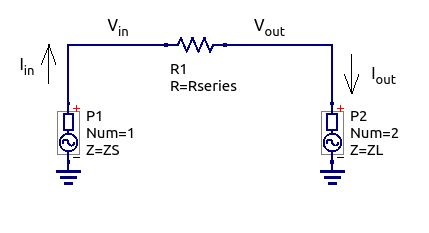
\includegraphics[width=10cm]{./images/r-series-attenuator-schematic.png}
    \caption{Series resistor attenuator}
    \label{fig:r-series-attenuator-schematic}
  \end{figure}

\noindent The design equations are derived more easily from the point of view of the power reflection and transmission rather than from the nodal analysis perspective. There are two interfaces where the impedance mismatch ocurr: the first one between the source and the series resistor and the second one between the series resistor and the load impedance.

\noindent In the interface between the source impedance and the resistor, the loss caused by the mismatch is given by:

\begin{equation}
	t_1 = 1 - \left| \frac{Z_S - (R + Z_L)}{Z_S + R + Z_L}\right|
\end{equation}  

\noindent Between the resistor and the load impendance, the loss caused by the mismatch is:

\begin{equation}
	t_2 = 1 - \left| \frac{(Z_S + R) - Z_L}{Z_S + R + Z_L}\right|
\end{equation} 

\noindent Consequently, the total power loss is:

\begin{equation}
	t = t_1 \cdot t_2 = \frac{4 \cdot Z_L \cdot Z_S}{R^2 + 2 \cdot R \cdot Z_L + Z_L^2 + 2 \cdot Z_S \cdot (R  + Z_L) + Z_S^2}
	\label{eq:r-series-power-loss}
\end{equation}

\noindent Eq. \ref{eq:r-series-power-loss} gives two solutions, but only one gives positive values:

\begin{equation}
	R = \frac{1}{\alpha^{n.u.}} \cdot \left( -\alpha^{n.u.} \cdot (Z_L + Z_S) + 2 \sqrt{Z_L \cdot Z_S \cdot \alpha^{n.u.}} \right)
\end{equation}
